\chapter{Diagramma di macchina a stati}
Le macchine a stati possono essere utilizzate per modellare il comportamento dinamico di classificatori
quali classi, casi d'uso, sottosistemi e interi sistemi.
\\ Le macchine a stati esistono nel contesto di un particolare classificatore che:
\begin{itemize}
    \item Risponde a eventi esterni
    \item Ha un ciclo di vita definito, che può essere modellato come una successione di stati,
    transizioni ed eventi
    \item Può avere un comportamento corrente che dipende dai comportamenti precedenti
\end{itemize}
Le macchine a stati di solito vengono utilizzate per modellare il comportamento
dinamico degli oggetti.
\section{Tipi di oggetti}
\begin{itemize}
    \item Indipendenti dallo stato - Oggeti che rispondono sempre nello statto modo a un determinato evento
    \item Dipendenti dallo stato - Rispondono in modi diversi ad un determinato evento a seconda dello stato
    in cui si trovano
\end{itemize}
\subsection*{Modellazione oggetti dipendenti dallo stato}
Modellano il comportamento di un oggetto reattivo complesso in risposta agli eventi oppure modellano
le sequenze valide delle operazioni ovvero specifiche di protocollo o linguaggio.
\\ Esempi di oggetti complessi sono dispositivi fisici come un telefono o un'auto, oppure
transazioni e oggetti di business (ordine, vendita, pagamenti, ecc.).
\paragraph*{Altri esempi}
\begin{itemize}
    \item Protocolli di comunicazione - TCP si comporta in maniera diversa a seconda dello stato in cui 
    la comunicazione si trova
    \item Flusso e navigazione delle pagine/finestre UI
    \item Controlle di flusso UI
    \item Operazioni di sistema dei casi d'uso - endSale deve arrivare solo dopo una o più operazioni enterItem
\end{itemize}
\section{Macchina a stati - Sintassi e rappresentazione}
Noterete dalla seguente immagine che si tratta praticamente di un DFA 
(Deterministic Finite Automa - Automa a stati finiti deterministico) dove abbiamo:
\begin{itemize}
    \item Uno stato iniziale
    \item Stati intermedi
    \item Transizioni (etichettate da eventi)
    \item Stato finale
\end{itemize}
\begin{center}
    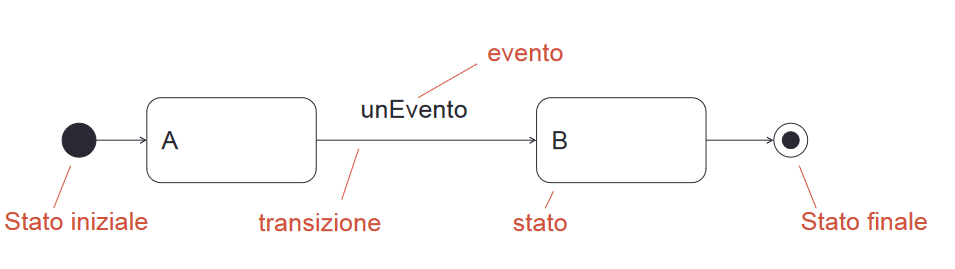
\includegraphics[scale=0.5, width=100mm]{img/macchina_a_stati_syntax.png}
\end{center}
\subsection*{Stati}
Una condizione o una situazione della vita di un oggetto durante la quale tale oggetto soddisfa
una condizione, esegue un'attività o aspetta un evento.
Lo stato di un oggetto in qualsiasi momento è determinato da
\begin{itemize}
    \item I valori dei suoi attributi
    \item Le relazioni che ha con altri oggetti
    \item Le attività che sta eseguendo
\end{itemize}
Le azioni sono istantanee e non interrompibili, le transizioni interne occorrono dentro
lo stato e non causano la transizione in un nuovo stato, mentre le attività richiedono un
intervallo di tempo finito e sono interrompibili.
\\ Le transizioni possono essere collegate tramite uno pseudo stato
di giunzione o tramite uno pseudo stato di selezione (tipo if else).
\subsection*{Eventi}
Gli \textbf{eventi} attivano le transizioni nelle macchine a stati.
\\ Ci sono eventi di diversa tipologia:
\paragraph*{Eventi di chiamata} Una chiamata per una specifica operazione.
L'evento dovrebbe avere la stessa segnatura di un'operazione della classe di contesto.
\paragraph*{Eventi di segnale} Un segnalte è un pacchetto di informazioni inviato in modo
asincrono tra oggetti. Non ha operazioni perchè il suo scopo è trasportare informazioni.
\paragraph*{Ricezione del segnale} indicata da un pentagono concavo.
\paragraph*{Evento di Variazione} Un evento di variazione è un'espressione booleana:
L'azione viene eseguita quando il valore dell'espressione passa da falso a vero.
Da un punto di vista implementativo, l'espressione viene valutata in modo periodico (ciclo di test continuo).
\paragraph*{Evento temporale} Un evento temporale è un evento che si verifica dopo un certo periodo di tempo,
quindi quando un'espressione di tempo diventa vera.
\subsection*{Stati composti}
Hanno una o più regioni ognuna delle quali contiene una sottomacchina annidata.
\\ Il più semplice contiene una sola regione, mentre quelli compositi ortogonali hanno
due o più regioni e quando si entra nello stato composito tutte le macchine iniziano la loro esecuzione
in modo concorrente. L'uiscta può essere sincronizzata, cioè si esce dallo stato quando tutte le regioni sono
terminate, oppure asincrona, cioè si esce dallo stato composito quando una regioen termina e l'altra
sottomacchine viene terminata.
\subsection*{Comunicazione tra sotto macchine}
Capita spesso di avere l'esigenza di far comunicare due sotto-macchine, biforcazioni e
ricongiuizioni possono essere usate per creare sotto-macchine concorrenti e per ri-sincronizzarle.
La comunicazione asincrona è ottenuta da una sotto-macchina configurando un flag per un'altra sotto-macchina.
\paragraph*{Stato di sync} Come alternativa all'utilizzo degli attributi possiamo utilizzare uno stato di sync
il cui compito è quello di tenere traccia di ogni singola attivazione della sua unica transizione di
input. Lo stato di sync è come se fosse una coda dove si aggiunge un elemento alla coda ogni volta
che viene attiva la transizione di input.
\subsection*{Stati con memoria semplice} 
Lo pseudo-stto con memoria semplice ricorda in quale sottostato si era quando si è lasciato il super stato,
in seguito quando si ritorna da uno stato esterno allo stato con memoria, l'indicatore ridirezione la 
transizione sull'ultimo sottostato memorizzato.
\paragraph*{Memoria multilivello} Uno stato con memoria multilivello può ricordarsi di più sottostati.
\section{I diagrammi di macchina in UP}
Non esiste nessun modello in UP chiamato "modello a stati", tuttavia qualsiasi elemento in qualsiasi modello
può avere una macchina a stati per comprendere o comunicare meglio il proprio comportamento dinamico.
\paragraph*{Esempio} Macchina a stati per rappresentare un processo di vendita, dalla selezione dell'item,
al pagamento.
\chapter{Diagramma di attività}
